\label{design:overview}
\label{sec:design_overview}
As part of a greater platform, the launcher is required to provide services to other components of the \giraf[] system, and may also depend on others.
The required services and dependencies are outlined below.

\autoref{fig:external_architecture} illustrates the \giraf[] launcher component. The component provides one service and has one dependency.
The service it provides is based on demands from the surrounding components of the \giraf[] platform, which can be seen in \autoref{fig:Giraf_comp_pic}.
The illustrated service provides a way for launched \girafapp[]s to determine which guardian launched the app in question, with which child profile, together with color data of the specific app.

Knowing which child profile the app in question was launched with is required, as the \giraf[] platform, as of writing, is designed for \emph{guardian mode} -- described in \autoref{backlog:guardian_mode} -- instead of \emph{child mode} -- described in \autoref{backlog:child_mode} -- or a combination hereof.

The illustrated dependency represents the need for being able to read and update profile data. The service which fulfills this dependency is provided by the Oasis lib. 

As seen on \autoref{fig:Giraf_comp_pic}, Oasis is available for the launcher to use. Oasis stores the modelled data, including the guardian and child profiles on the device in a local database.


\begin{figure}[h]
	\centering
	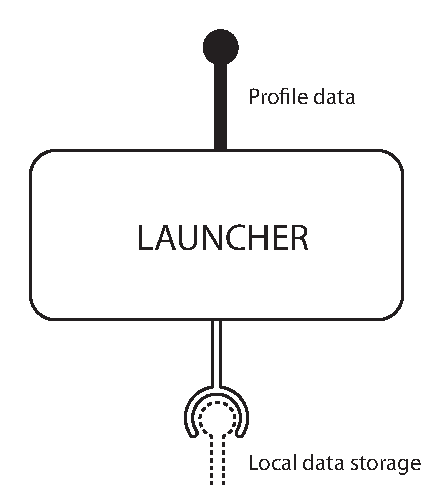
\includegraphics[width=0.5\textwidth]{gfx/external_launcher_architecture.pdf}
	\caption{The \giraf[] launcher component.}
	\label{fig:external_architecture}
\end{figure}

Being able to launch a \girafapp[] as a specific guardian requires the user to interact such that the launcher knows which guardian the user represents.

Authentication was chosen, as each modulated child and guardian contains private data and therefore need to be protected.

\begin{figure}[h]
	\centering
	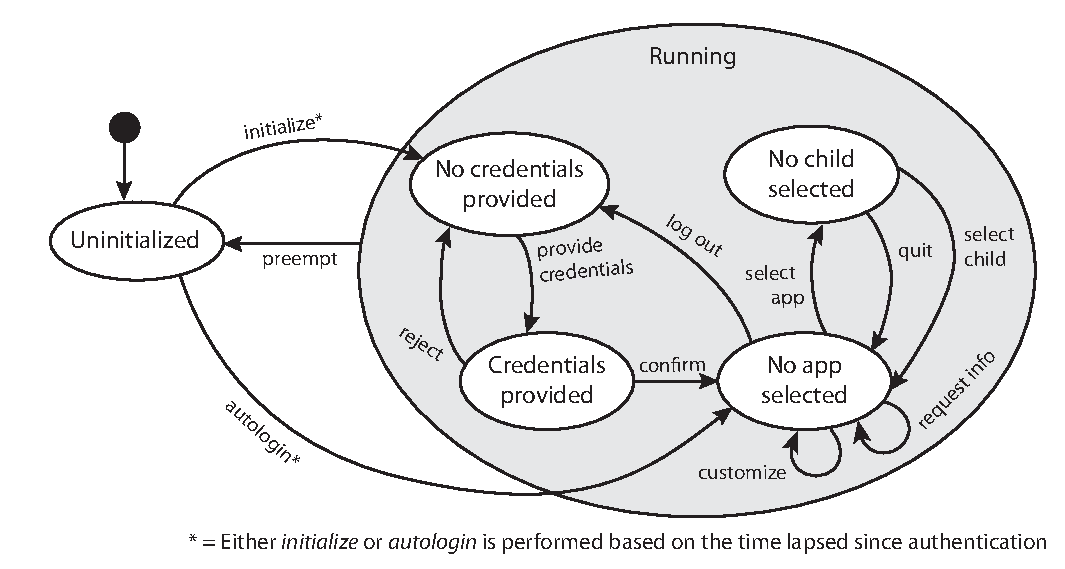
\includegraphics[width=1\textwidth]{gfx/statediagram.pdf}
	\caption{State diagram}
	\label{fig:state_diagram}
\end{figure}


\autoref{fig:state_diagram} shows all possible states and transitions, which the launcher can be in. 
These states grouped together represent four functionalities of the launcher:

\begin{enumerate}
	\item Initialization
	\item Authentication
	\item App management
	\item Profile selection
\end{enumerate}

These functionalities are shown in \autoref{fig:design_diagram}, along with the states they represent, and the transitions between them.

\begin{figure}[h!]
	\centering
	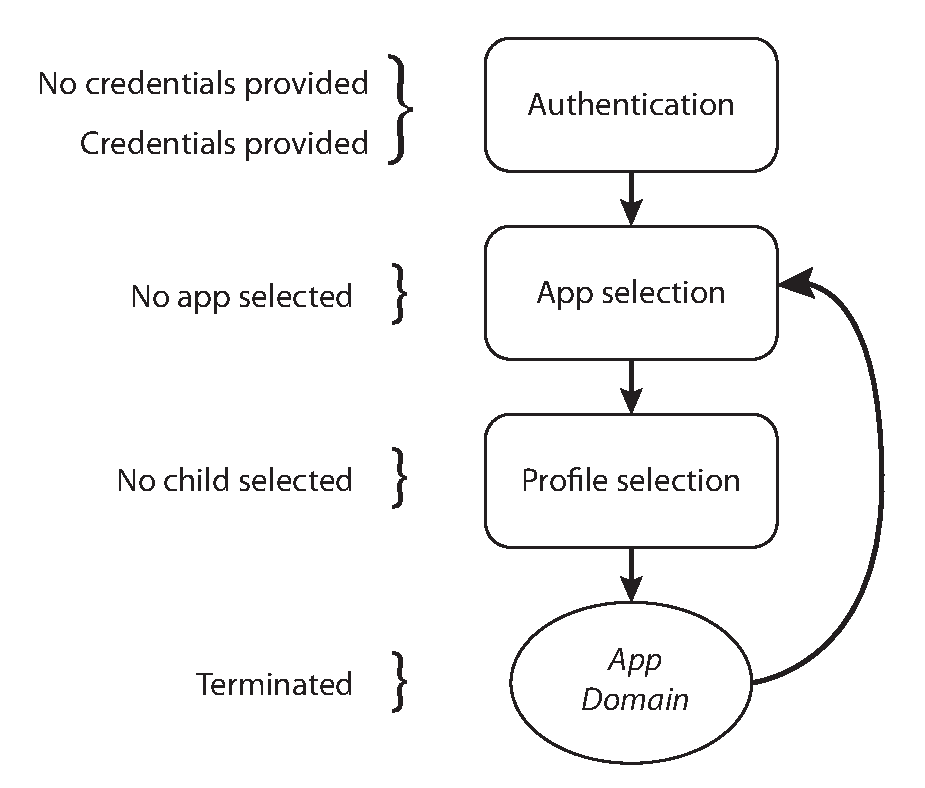
\includegraphics[width=1\textwidth]{gfx/design_diagram.pdf}
	\caption{Functionality diagram}
	\label{fig:design_diagram}
\end{figure}

The states, transitions and functionalities, are explained below in their appropriate sections.

In order to highten usability, as requested by the customers in \autoref{interviews}, it is decided to standardize elements in the GUI. These standards together are referred to as the \emph{design language}.
Furthermore, it is decided that the concrete elements are to be shared, such that other \giraf[] components can utilize the standards.

\begin{figure}[h!]
	\centering
	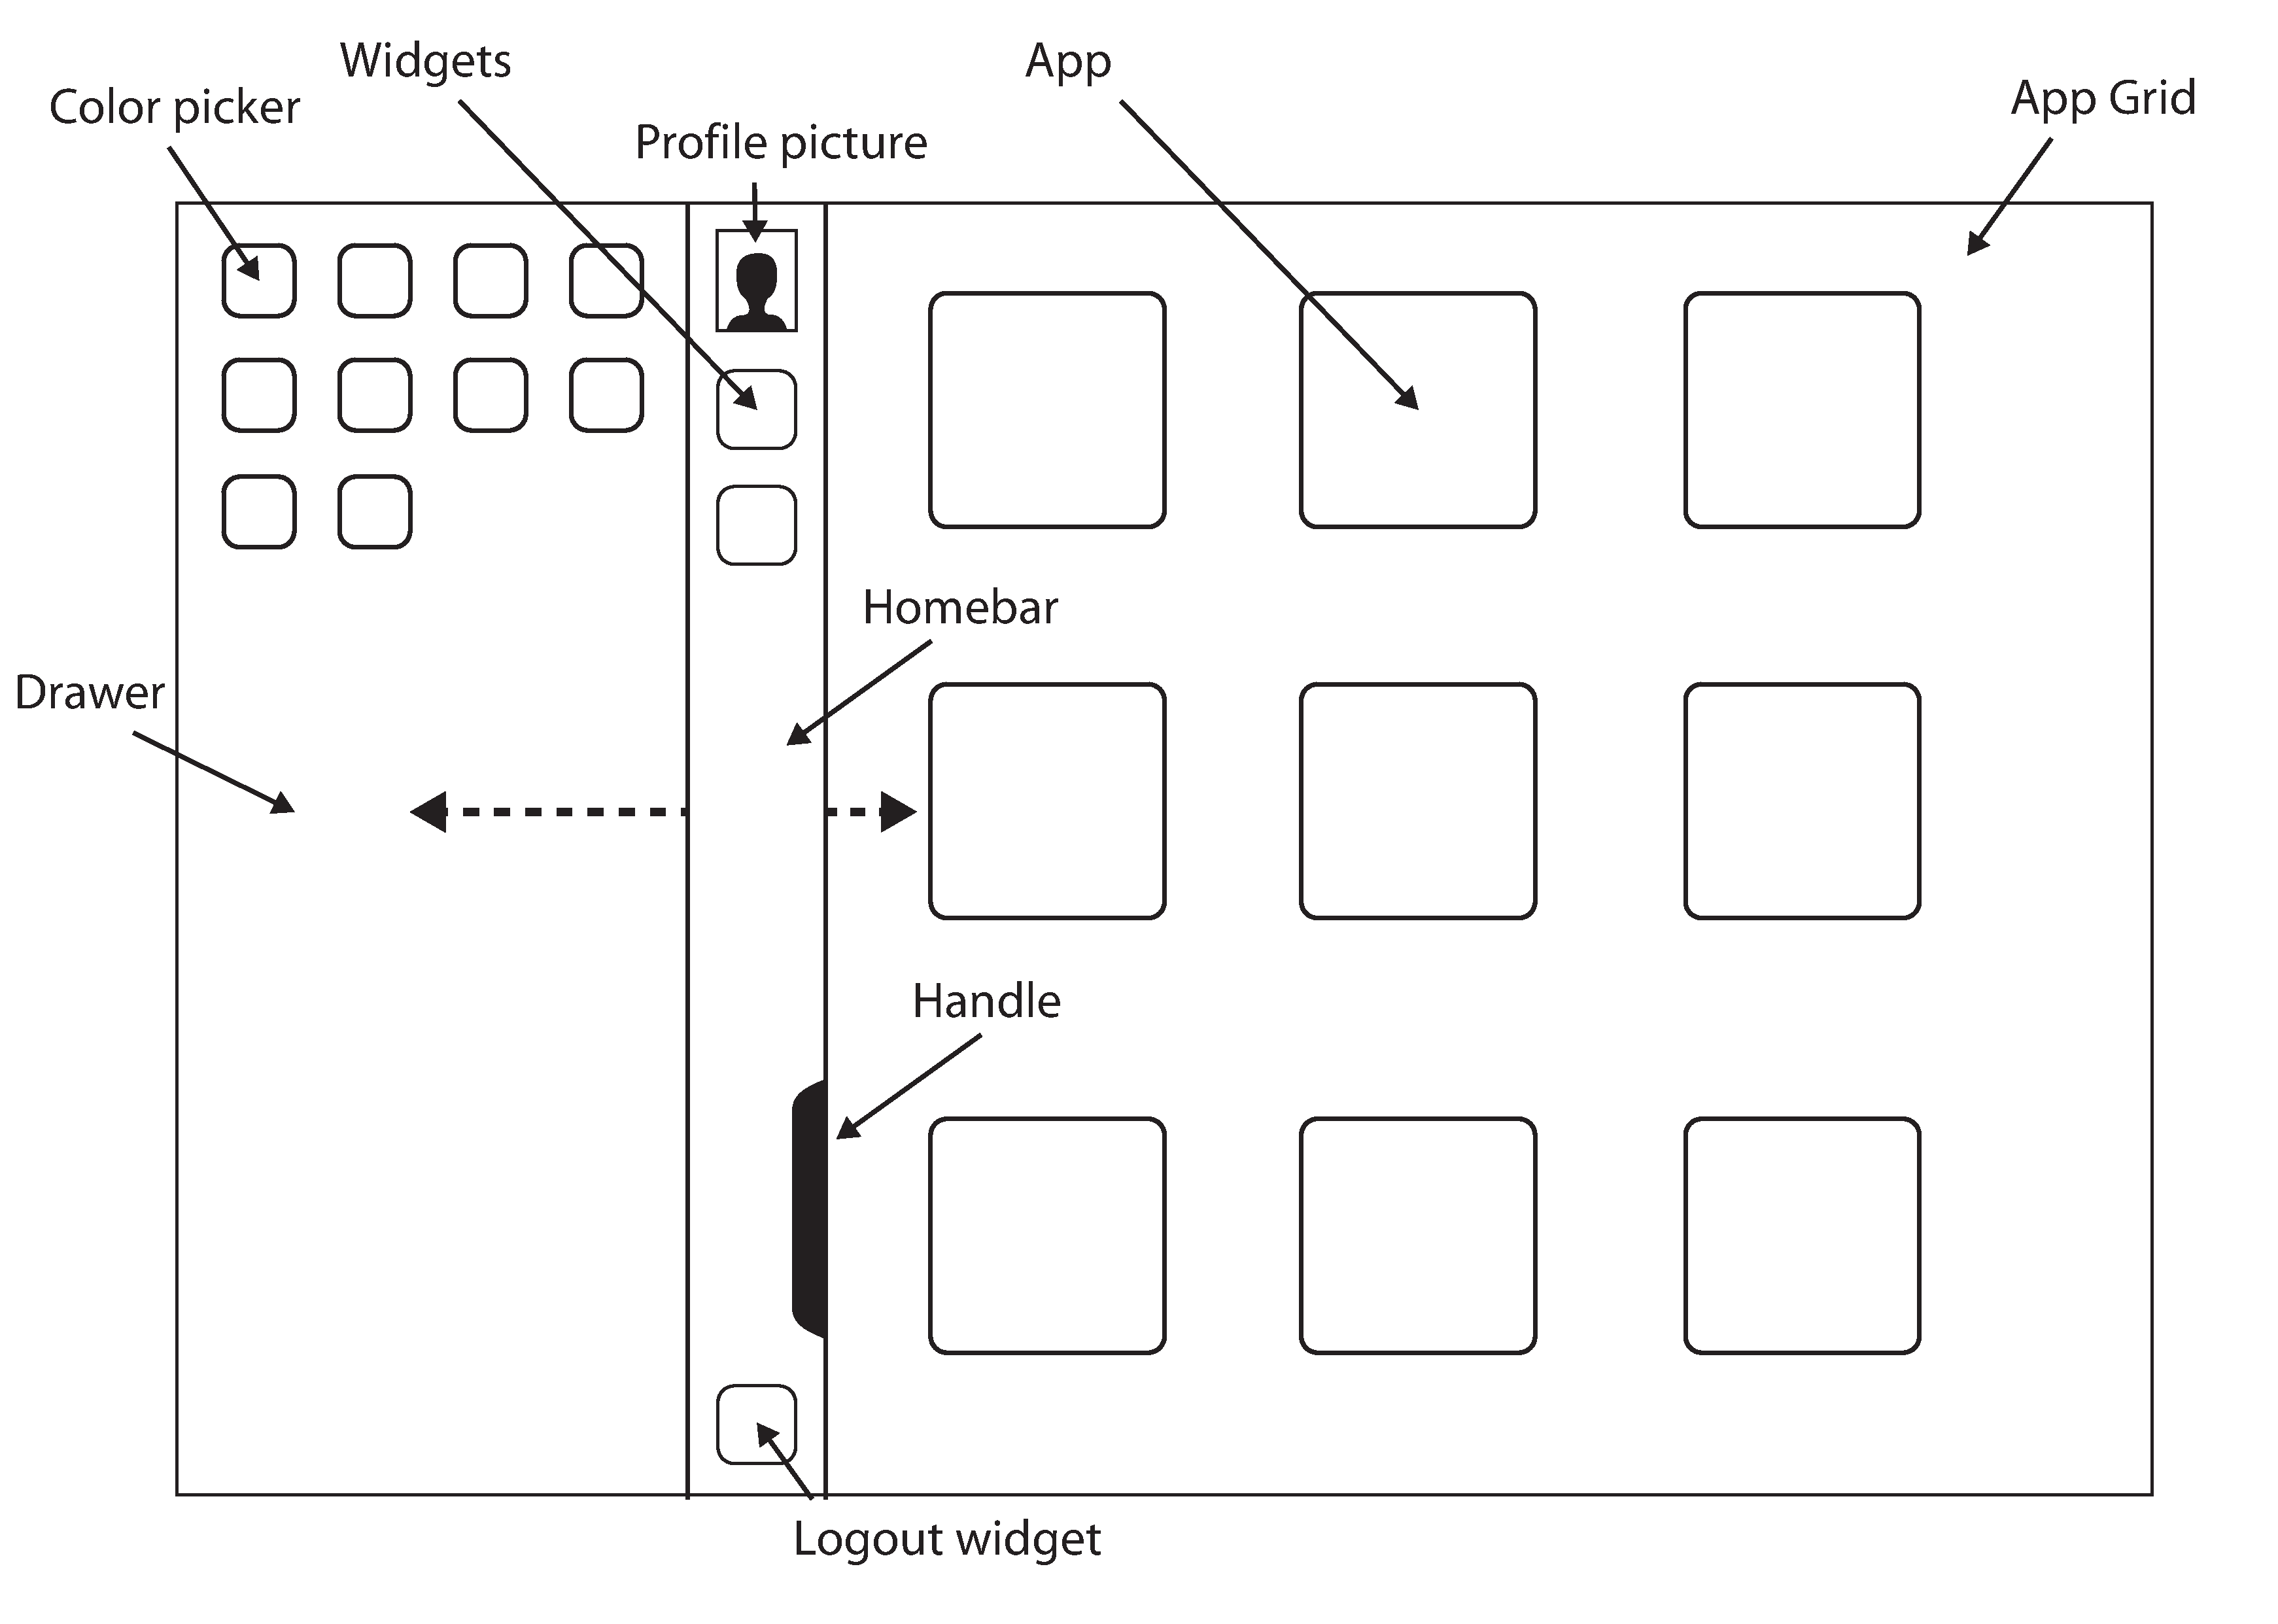
\includegraphics[width=1\textwidth]{gfx/design_prototype.pdf}
	\caption{Design prototype}
	\label{fig:design_prototype}
\end{figure}

\autoref{fig:design_prototype} shows the overall design which will be explained in this chapter and with commen names on all elements of greater importance.